\documentclass[12pt,a4paper]{article}

%%%%%% LINE SPACING %%%%%%%%%%%%
\usepackage{setspace}
\singlespacing
%\onehalfspacing
%\doublespacing

%Define a test for doing PDF format -- use different code below
\newif\ifPDF
\ifx\pdfoutput\undefined\PDFfalse 
\else\ifnum\pdfoutput > 0\PDFtrue 
     \else\PDFfalse 
     \fi 
\fi

\textwidth=161 mm
\textheight=245 mm
\topmargin=-15 mm
\oddsidemargin=0 mm
\parindent=6 mm

\usepackage[sort]{natbib}
\usepackage{lscape}
\bibpunct[,]{(}{)}{;}{a}{}{,}

\newcommand{\eg}{e.g.\ }
\newcommand{\ie}{i.e.\ }
\newcommand{\hi}{H{\sc i}}
\newcommand{\hipass}{{\sc hipass}}
\newcommand{\duchamp}{\emph{Duchamp}}
\newcommand{\atrous}{\textit{{\`a} trous}}
\newcommand{\Atrous}{\textit{{\`A} trous}}
\newcommand{\diff}{{\rm d}}
\newcommand{\entrylabel}[1]{\mbox{\textsf{\bf{#1:}}}\hfil}
\newenvironment{entry}
        {\begin{list}{}%
                {\renewcommand{\makelabel}{\entrylabel}%
                        \setlength{\labelwidth}{30mm}%
                        \setlength{\labelsep}{5pt}%
                        \setlength{\itemsep}{2pt}%
                        \setlength{\parsep}{2pt}%
                        \setlength{\leftmargin}{35mm}%
                }%
        }%
{\end{list}}


\title{Source Detection with \duchamp\ v1.0\\A User's Guide}
\author{Matthew Whiting\\
Australia Telescope National Facility\\CSIRO}
\date{}

% If we are creating a PDF, use different options for graphicx, hyperref.
\ifPDF
  \usepackage[pdftex]{graphicx,color}
  \usepackage[pdftex]{hyperref}
  \hypersetup{colorlinks=true,% 	    
              citecolor=red,%
              filecolor=red,%
              linkcolor=red,%
              urlcolor=red,%
              }
\else
  \usepackage[dvips]{graphicx} 
  \usepackage[dvips]{hyperref} 
\fi

\pagestyle{headings}
\begin{document}

\maketitle
\thispagestyle{empty}
\begin{figure}[!h]
\begin{center}
\includegraphics[width=\textwidth]{cover_image}
\end{center}
\end{figure}

\newpage
\tableofcontents

\newpage
\section{Introduction and getting going quickly}

This document provides a user's guide to \duchamp, an object-finder
for use on spectral-line data cubes. The basic execution of
\duchamp\ is to read in a FITS data cube, find sources in the cube,
and produce a text file of positions, velocities and fluxes of the
detections, as well as a postscript file of the spectra of each
detection.

So, you have a FITS cube, and you want to find the sources in it. What
do you do? The first step is to make an input file that contains the
list of parameters. Brief and detailed examples are shown in
Appendix~\ref{app-input}. This file provides the input file name, the various
output files, and defines various parameters that control the
execution.

The standard way to run \duchamp\ is by the command
\begin{quote}
\texttt{Duchamp -p [parameter file]}
\end{quote}
replacing \texttt{[parameter file]} with the name of the file listing
the parameters. Alternatively, you can use the syntax
\begin{quote}
\texttt{Duchamp -f [FITS file]}
\end{quote}
where \texttt{[FITS file]} is the file you wish to search. In the latter
case, all parameters will take their default values detailed in
Appendix~\ref{app-param}. In either case, the program will then work
away and give you the list of detections and their spectra. The
program execution is summarised below, and detailed in
\S\ref{sec-flow}. Information on inputs is in \S\ref{sec-param} and
Appendix~\ref{app-param}, and descriptions of the output is in
\S\ref{sec-output}.

\subsection{A summary of the execution steps}

The basic flow of the program is summarised here -- all steps are
discussed in more detail in the following sections.
\begin{enumerate}
\item If the \texttt{-p} option is used, the parameter file given on
  the command line is read in, and the parameters absorbed.
\item The FITS image is located and read in to memory.
\item If requested, a FITS image with a previously reconstructed array
  is read in.
\item If requested, blank pixels are trimmed from the edges, and
  the baseline of each spectrum is removed.
\item If the reconstruction method is requested, and the reconstructed
  array has not been read in at Step 3 above, the cube is
  reconstructed using the \atrous\ wavelet method.
\item Searching for objects then takes place, using the requested
  thresholding method.
\item The list of objects is condensed by merging neighbouring objects
  and removing those deemed unacceptable.
\item The baselines and trimmed pixels are replaced prior to output.
\item The details of the detections are written to screen and to the
  requested output file.
\item Maps showing the spatial location of the detections are written.
\item The integrated spectra of each detection are written to a
  postscript file. 
\item If requested, the reconstructed array can be written to a new
  FITS file.
\end{enumerate}

\subsection{Guide to terminology}

First, a brief note on the use of terminology in this guide. \duchamp\
is designed to work on FITS ``cubes''. These are FITS\footnote{FITS is
the Flexible Image Transport System -- see \citet{hanisch01} or
websites such as 
\href{http://fits.cv.nrao.edu/FITS.html}{http://fits.cv.nrao.edu/FITS.html}
for details.} image arrays with three dimensions -- they are assumed
to have the following form: the first two dimensions (referred to as
$x$ and $y$) are spatial directions (that is, relating to the position
on the sky), while the third dimension, $z$, is the spectral
direction, which can correspond to frequency, wavelength, or
velocity. The three dimensional analogue of pixels are ``voxels'', or
volume cells -- a voxel is defined by a unique $(x,y,z)$ location and
has a unique flux or intensity value associated with it.

Each spatial pixel (a given $(x,y)$ coordinate) can be said to be a
single spectrum, while a slice through the cube perpendicular to the
spectral direction at a given $z$-value is a single channel (the 2-D
image is a channel map).

Detection involves locating a contiguous group of voxels with fluxes
above a certain threshold. \duchamp\ makes no assumptions as to the
size or shape of the detected features, other than having
user-selected minimum size criteria.

Features that are detected are assumed to be positive. The user can
choose to search for negative features by setting an input parameter
-- this inverts the cube prior to the search (see
\S\ref{sec-detection} for details).

Note that it is possible to run \duchamp\ on a two-dimensional image
(\ie one with no frequency or velocity information), or indeed a
one-dimensional array, and many of the features of the program will
work fine. The focus, however, is on object detection in three
dimensions.

\subsection{Why \duchamp?}

Well, it's important for a program to have a name, and the initial
working title of \emph{cubefind} was somewhat uninspiring. I wanted to
avoid the classic astronomical approach of designing a cute acronym,
and since it is designed to work on cubes, I looked at naming it after
a cubist. \emph{Picasso}, sadly, was already taken \citep{minchin99},
so I settled on naming it after Marcel Duchamp, another cubist, but
also one of the first artists to work with ``found objects''.

\section{User Inputs}
\label{sec-param}

Input to the program is provided by means of a parameter
file. Parameters are listed in the file, followed by the value that
should be assigned to them. The syntax used is \texttt{paramName
value}. Parameter names are not case-sensitive, and lines in the input
file that start with \texttt{\#} are ignored. If a parameter is listed
more than once, the latter value is used, but otherwise the order in
which the parameters are listed in the input file is
arbitrary. Example input files can be seen in
Appendix~\ref{app-input}.

If a parameter is not listed, the default value is assumed. The
defaults are chosen to provide a good result (using the reconstruction
method), so the user doesn't need to specify many new parameters in
the input file. Note that the image file \textbf{must} be specified! The
parameters that can be set are listed in Appendix~\ref{app-param},
with their default values in parentheses.

The parameters with names starting with \texttt{flag} are stored as
\texttt{bool} variables, and so are either \texttt{true = 1} or
\texttt{false = 0}. They can be entered in the file either in text or
integer format -- \duchamp\ will read them correctly in either case. 

\section{What \duchamp\ is doing}
\label{sec-flow}

The execution flow of \duchamp\ is detailed here, indicating the
main algorithmic steps that are used. The program is written in C/C++
and makes use of the {\sc cfitsio}, {\sc wcslib} and {\sc pgplot}
libraries. 

\subsection{Image input}
\label{sec-input}

The cube is read in using basic {\sc cfitsio} commands, and stored as
an array in a special C++ class. This class keeps track of
the list of detected objects, as well as any reconstructed arrays that
are made (see \S\ref{sec-recon}). The World Coordinate System (WCS)
information for the cube is also obtained from the FITS header by {\sc
wcslib} functions \citep{greisen02, calabretta02}, and this
information, in the form of a \texttt{wcsprm} structure, is also stored
in the same class.

A sub-section of an image can be requested via the \texttt{subsection}
parameter in the parameter file -- this can be a good idea if the cube
has very noisy edges, which may produce many spurious detections. The
generalised form of the subsection that is used by {\sc cfitsio} is
\texttt{[x1:x2:dx,y1:y2:dy,z1:z2:dz]}, such that the x-coordinates run
from \texttt{x1} to \texttt{x2} (inclusive), with steps of
\texttt{dx}. The step value can be omitted (so a subsection of the
form \texttt{[2:50,2:50,10:1000]} is still valid). \duchamp\ does not
make use of any step value present in the subsection string, and any
that are present are removed before the file is opened.

If one wants the full range of a coordinate then replace the range
with an asterisk, \eg \texttt{[2:50,2:50,*]}. If one wants to use a
subsection, one must set \texttt{flagSubsection = 1}. A complete
description of the section syntax can be found at the {\sc fitsio} web
site
\footnote{
\href{http://heasarc.gsfc.nasa.gov/docs/software/fitsio/c/c\_user/node90.html}%
{http://heasarc.gsfc.nasa.gov/docs/software/fitsio/c/c\_user/node90.html}}.

\subsection{Image modification}
\label{sec-modify}

Several modifications to the cube can be made that improve the
execution and efficiency of \duchamp\ (these are optional -- their
use is indicated by the relevant flags set in the input parameter
file).

\subsubsection{Blank pixel removal}

First, the cube is trimmed of any BLANK pixels that pad the image out
to a rectangular shape. This is optional, its use determined by the
\texttt{flagBlankPix} parameter. The value for these pixels is read from
the FITS header (using the BLANK, BSCALE and BZERO keywords), but if
these are not present then the value can be specified by the user in
the parameter file using \texttt{blankPixValue}.

This stage is particularly important for the reconstruction step, as
lots of BLANK pixels on the edges will smooth out features in the
wavelet calculation stage. The trimming will also reduce the size of
the cube's array, speeding up the execution. The amount of trimming is
recorded, and these pixels are added back in once the source-detection
is completed (so that quoted pixel positions are applicable to the
original cube).

Rows and columns are trimmed one at a time until the first non-BLANK
pixel is reached, so that the image remains rectangular. In practice,
this means that there will be BLANK pixels left in the trimmed image
(if the non-BLANK region is non-rectangular). However, these are
ignored in all further calculations done on the cube.

\subsubsection{Baseline removal}

Second, the user may request the removal of baselines from the
spectra, via the parameter \texttt{flagBaseline}. This may be necessary
if there is a strong baseline ripple present, which can result in
spurious detections at the high points of the ripple. The baseline is
calculated from a wavelet reconstruction procedure (see
\S\ref{sec-recon}) that keeps only the two largest scales. This is
done separately for each spatial pixel (\ie for each spectrum in the
cube), and the baselines are stored and added back in before any
output is done. In this way the quoted fluxes and displayed spectra
are as one would see from the input cube itself -- even though the
detection (and reconstruction if applicable) is done on the
baseline-removed cube.

The presence of very strong signals (for instance, masers at several
hundred Jy) can affect the determination of the baseline, leading to a
large dip centred on the signal in the baseline-subtracted
spectrum. To prevent this, the signal is trimmed prior to the
reconstruction process at some standard threshold (at $8\sigma$ above
the mean). The baseline determined should thus be representative of
the true, signal-free baseline. Note that this trimming is only a
temporary measure which does not affect the source-detection.

\subsubsection{Ignoring bright Milky Way emission}

Finally, a single set of contiguous channels can be ignored -- these
may exhibit very strong emission, such as that from the Milky Way as
seen in extragalactic \hi\ cubes (hence the references to ``Milky
Way'' in relation to this task -- apologies to Galactic
astronomers!). Such dominant channels will produce many detections
that are unnecessary, uninteresting (if one is interested in
extragalactic \hi) and large (in size and hence in memory usage), and
so will slow the program down and detract from the interesting
detections. The use of this feature is controlled by the
\texttt{flagMW} parameter, and the exact channels concerned are able
to be set by the user (using \texttt{maxMW} and \texttt{minMW} --
these give an inclusive range of channels). When employed, these
channels are temporarily blanked out for the searching, and the
scaling of the spectral output (see Fig.~\ref{fig-spect}) will not
take them into account. They will be present in the reconstructed
array, however, and so will be included in the saved FITS file (see
\S\ref{sec-reconIO}). When the final spectra are plotted, the range of
channels covered by these parameters is indicated by a green hashed
box.

\subsection{Image reconstruction}
\label{sec-recon}

The user can direct \duchamp\ to reconstruct the data cube using the
\atrous\ wavelet procedure. A good description of the procedure can be
found in \citet{starck02:book}. The reconstruction is an effective way
of removing a lot of the noise in the image, allowing one to search
reliably to fainter levels, and reducing the number of spurious
detections. This is an optional step, but one that greatly enhances
the source-detection process, with the payoff that it can be
relatively time- and memory-intensive.

\subsubsection{Algorithm}

The steps in the \atrous\ reconstruction are as follows:
\begin{enumerate}
\item Set the reconstructed array to 0 everywhere.
\item The input array is discretely convolved with a given filter
  function. This is determined from the parameter file via the
  \texttt{filterCode} parameter -- see Appendix~\ref{app-param} for
  details on the filters available.
\item The wavelet coefficients are calculated by taking the difference
  between the convolved array and the input array.
\item If the wavelet coefficients at a given point are above the
  requested threshold (given by \texttt{snrRecon} as the number of
  $\sigma$ above the mean and adjusted to the current scale -- see
  Appendix~\ref{app-scaling}), add these to the reconstructed array.
\item The separation of the filter coefficients is doubled. (Note that
  this step provides the name of the procedure\footnote{\atrous\ means
  ``with holes'' in French.}, as gaps or holes are created in the
  filter coverage.)
\item The procedure is repeated from step 2, using the convolved array
  as the input array.
\item Continue until the required maximum number of scales is reached.
\item Add the final smoothed (\ie convolved) array to the
  reconstructed array. This provides the ``DC offset'', as each of the
  wavelet coefficient arrays will have zero mean.
\end{enumerate}

The reconstruction has at least two iterations. The first iteration
makes a first pass at the wavelet reconstruction (the process outlined
in the 8 stages above), but the residual array will inevitably have
some structure still in it, so the wavelet filtering is done on the
residual, and any significant wavelet terms are added to the final
reconstruction. This step is repeated until the change in the $\sigma$
of the background is less than some fiducial amount.

It is important to note that the \atrous\ decomposition is an
example of a ``redundant'' transformation. If no thresholding is
performed, the sum of all the wavelet coefficient arrays and the final
smoothed array is identical to the input array. The thresholding thus
removes only the unwanted structure in the array.

Note that any BLANK pixels that are still in the cube will not be
altered by the reconstruction -- they will be left as BLANK so that
the shape of the valid part of the cube is preserved.

\subsubsection{Note on Statistics}

The correct calculation of the reconstructed array needs good
estimation of the underlying mean and standard deviation of the
background noise distribution. These statistics are estimated using
robust methods, to avoid corruption by strong outlying points. The
mean of the distribution is actually estimated by the median, while
the median absolute deviation from the median (MADFM) is calculated
and corrected assuming Gaussianity to estimate the underlying standard
deviation $\sigma$. The Gaussianity (or Normality) assumption is
critical, as the MADFM does not give the same value as the usual rms
or standard deviation value -- for a normal distribution
$N(\mu,\sigma)$ we find MADFM$=0.6744888\sigma$. The difference
between the MADFM and $\sigma$ is corrected for, so the user need only
think in the usual multiples of $\sigma$ when setting
\texttt{snrRecon}. See Appendix~\ref{app-madfm} for a derivation of
this value.

When thresholding the different wavelet scales, the value of $\sigma$
as measured from the wavelet array needs to be scaled to account for the
increased amount of correlation between neighbouring pixels (due to
the convolution). See Appendix~\ref{app-scaling} for details on this
scaling. 

\subsubsection{User control of reconstruction parameters}

The most important parameter for the user to select in relation to the
reconstruction is the threshold for each wavelet array. This is set
using the \texttt{snrRecon} parameter, and is given as a multiple of the
rms (estimated by the MADFM) above the mean (which for the wavelet
arrays should be approximately zero). There are several other
parameters that can be altered as well that affect the outcome of the
reconstruction. 

By default, the cube is reconstructed in three dimensions, using a
3-dimensional filter and 3-dimensional convolution. This can be
altered, however, using the parameter \texttt{reconDim}. If set to 1,
this means the cube is reconstructed by considering each spectrum
separately, whereas \texttt{reconDim=2} will mean the cube is
reconstructed by doing each channel map separately. The merits of
these choices are discussed in \S\ref{sec-notes}, but it should be
noted that a 2-dimensional reconstruction can be susceptible to edge
effects if the spatial shape is not rectangular.

The user can also select the minimum scale to be used in the
reconstruction -- the first scale exhibits the highest frequency
variations, and so ignoring this one can sometimes be beneficial in
removing excess noise. The default, however, is to use all scales
(\texttt{minscale = 1}). 

Finally, the filter that is used for the convolution can be selected
by using \texttt{filterCode} and the relevant code number -- the
choices are listed in Appendix~\ref{app-param}. A larger filter will
give a better reconstruction, but take longer and use more memory when
executing. When multi-dimensional reconstruction is selected, this
filter is used to construct a 2- or 3-dimensional equivalent.

\subsection{Reconstruction I/O}
\label{sec-reconIO}

The reconstruction stage can be relatively time-consuming, particularly 
for large cubes and reconstructions in 3-D. To get around this, \duchamp\ 
provides a shortcut to allow users to perform multiple searches (\eg with 
different thresholds) on the same reconstruction without calculating the 
reconstruction each time.

The first step is to choose to save the reconstructed array as a FITS 
file by setting \texttt{flagOutputRecon = true}. The file will be saved 
in the same directory as the input image, so the user needs to have write 
permissions for that directory.

The filename will be derived from the input filename, with extra
information detailing the reconstruction that has been done. For
example, suppose \texttt{image.fits} has been reconstructed using a
3-dimensional reconstruction with filter 2, thresholded at $4\sigma$
using all scales. The output filename will then be
\texttt{image.RECON-3-2-4-1.fits} (\ie it uses the four parameters
relevant for the \atrous\ reconstruction as listed in
Appendix~\ref{app-param}). The new FITS file will also have these
parameters as header keywords. If a subsection of the input image has
been used (see \S\ref{sec-input}), the format of the output filename
will be \texttt{image.sub.RECON-3-2-4-1.fits}, and the subsection that
has been used is also stored in the FITS header.

Likewise, the residual image, defined as the difference between the input 
and reconstructed arrays, can also be saved in the same manner by setting 
\texttt{flagOutputResid = true}. Its filename will be the same as above, 
with RESID replacing RECON.

If a reconstructed image has been saved, it can be read in and used
instead of redoing the reconstruction. To do so, the user should set
\texttt{flagReconExists = true}. The user can indicate the name of the
reconstructed FITS file using the \texttt{reconFile} parameter, or, if
this is not specified, \duchamp\ searches for the file with the name
as defined above. If the file is not found, the reconstruction is
performed as normal. Note that to do this, the user needs to set
\texttt{flagAtrous = true} (obviously, if this is \texttt{false}, the
reconstruction is not needed).

\subsection{Searching the image}
\label{sec-detection}

The image is searched for detections in two ways: spectrally (a
1-dimensional search in the spectrum in each spatial pixel), and
spatially (a 2-dimensional search in the spatial image in each
channel). In both cases, the algorithm finds connected pixels that are
above the user-specified threshold. In the case of the spatial image
search, the algorithm of \citet{lutz80} is used to raster scan through
the image and connect groups of pixels on neighbouring rows.

Note that this algorithm cannot be applied directly to a 3-dimensional
case, as it requires that objects are completely nested in a row: that
is, if you are scanning along a row, and one object finishes and
another starts, you know that you will not get back to the first one
(if at all) until the second is completely finished for that
row. Three-dimensional data does not have this property, which is why
we break up the searching into 1- and 2-dimensional cases.

The determination of the threshold is done in one of two ways. The
first way is a simple sigma-clipping, where a threshold is set at a
fixed number $n$ of standard deviations above the mean, and pixels
above this threshold are flagged as detected. The value of $n$ is set
with the parameter \texttt{snrCut}. As before, the value of the
standard deviation is estimated by the MADFM, and corrected by the
ratio derived in Appendix~\ref{app-madfm}.

The second method uses the False Discovery Rate (FDR) technique
\citep{miller01,hopkins02}, whose basis we briefly detail here. The
false discovery rate (given by the number of false detections divided
by the total number of detections) is fixed at a certain value
$\alpha$ (\eg $\alpha=0.05$ implies 5\% of detections are false
positives). In practice, an $\alpha$ value is chosen, and the ensemble
average FDR (\ie $\langle FDR \rangle$) when the method is used will
be less than $\alpha$.  One calculates $p$ -- the probability,
assuming the null hypothesis is true, of obtaining a test statistic as
extreme as the pixel value (the observed test statistic) -- for each
pixel, and sorts them in increasing order. One then calculates $d$
where
\[
d = \max_j \left\{ j : P_j < \frac{j\alpha}{c_N N} \right\},
\]
and then rejects all hypotheses whose $p$-values are less than or equal
to $P_d$. (So a $P_i<P_d$ will be rejected even if $P_i \geq
j\alpha/c_N N$.) Note that ``reject hypothesis'' here means ``accept
the pixel as an object pixel'' (\ie we are rejecting the null
hypothesis that the pixel belongs to the background). 

The $c_N$ values here are normalisation constants that depend on the
correlated nature of the pixel values. If all the pixels are
uncorrelated, then $c_N=1$. If $N$ pixels are correlated, then their
tests will be dependent on each other, and so $c_N = \sum_{i=1}^N
i^{-1}$. \citet{hopkins02} consider real radio data, where the pixels
are correlated over the beam. In this case the sum is made over the
$N$ pixels that make up the beam. The value of $N$ is calculated from
the FITS header (if the correct keywords -- BMAJ, BMIN -- are not
present, a default value of 10 pixels is assumed).

The theory behind the FDR method implies a direct connection between the 
choice of $\alpha$ and the fraction of detections that will be false 
positives. However, due to the merging process, this direct connection is
lost when looking at the final number of detections -- see discussion in
\S\ref{sec-notes}. The effect is that the number of false detections will
be less than indicated by the $\alpha$ value used.

If a reconstruction has been made, the residuals (defined as original
$-$ reconstruction) are used to estimate the noise parameters of the
cube. Otherwise they are estimated directly from the cube itself. In
both cases, robust estimators are used as described above.

Detections must have a minimum number of pixels to be counted. This
minimum number is given by the input parameters \texttt{minPix} (for
2-dimensional searches) and \texttt{minChannels} (for 1-dimensional
searches).

The search only looks for positive features. If one is interested
instead in negative features (such as absorption lines), set the
parameter \texttt{flagNegative = true}. This will invert the cube (\ie
multiply all pixels by $-1$) prior to the search, and then re-invert
the cube (and the fluxes of any detections) after searching is
complete. All outputs are done in the same manner as normal, so that
fluxes of detections will be negative.

\subsection{Merging detected objects}
\label{sec-merger}

The searching step produces a list of detected objects that will have many
repeated detections of a given object -- for instance, spectral
detections in adjacent pixels of the same object and/or spatial
detections in neighbouring channels. These are then combined in an
algorithm that matches all objects judged to be ``close''. This
determination is made in one of two ways.

One way is to define two thresholds -- one spatial and one in velocity
-- and say that two objects should be merged if there is at least one
pair of pixels that lie within these threshold distances of each
other. These thresholds are specified by the parameters
\texttt{threshSpatial} and \texttt{threshVelocity} (in units of pixels
and channels respectively).

Alternatively, the spatial requirement can be changed to say that
there must be a pair of pixels that are \emph{adjacent} -- a stricter,
but perhaps more realistic requirement, particularly when the spatial pixels
have a large angular size (as is the case for \hi\ surveys). This
method can be selected by setting the parameter
\texttt{flagAdjacent} to 1 (\ie \texttt{true}) in the parameter file. The
velocity thresholding is done in the same way as the first option.

Once the detections have been merged, they may be ``grown''. This is a
process of increasing the size of the detection by adding adjacent
pixels that are above some secondary threshold. This threshold is
lower than the one used for the initial detection, but above the noise
level, so that faint pixels are only detected when they are close to a
bright pixel. The value of this threshold is a possible input
parameter (\texttt{growthCut}), with a default value of $1.5\sigma$. The
use of the growth algorithm is controlled by the \texttt{flagGrowth}
parameter -- the default value of which is \texttt{false}. If the
detections are grown, they are sent through the merging algorithm a
second time, to pick up any detections that now overlap or have grown
over each other.

Finally, to be accepted, the detections must span \emph{both} a minimum
number of channels (to remove any spurious single-channel spikes that
may be present), and a minimum number of spatial pixels. These
numbers, as for the original detection step, are set with the
\texttt{minChannels} and \texttt{minPix} parameters. The channel
requirement means there must be at least one set of \texttt{minChannels}
consecutive channels in the source for it to be accepted.

\section{Outputs}
\label{sec-output}

\subsection{During execution}

\duchamp\ provides the user with feedback whilst it is running, to
keep the user informed on the progress of the analysis. Most of this
consists of self-explanatory messages about the particular stage the
program is up to. The relevant parameters are printed to the screen at
the start (once the file has been successfully read in), so the user
is able to make a quick check that the setup is correct (see
Appendix~{app-input} for an example).

If the cube is being trimmed (\S\ref{sec-modify}), the resulting
dimensions are printed to indicate how much has been trimmed. If a
reconstruction is being done, a continually updating message shows
either the current iteration and scale, compared to the maximum scale
(when \texttt{reconDim=3}), or a progress bar showing the amount of
the cube that has been reconstructed (for smaller values of
\texttt{reconDim}).

During the searching algorithms, the progress through the 1D and 2D
searches are shown. When the searches have completed,
the number of objects found in both the 1D and 2D searches are
reported (see \S\ref{sec-detection} for details).

In the merging process (where multiple detections of the same object
are combined -- see \S\ref{sec-merger}), two stages of output
occur. The first is when each object in the list is compared with all
others. The output shows two numbers: the first being how far through
the list the current object is, and the second being the length of the
list. As the algorithm proceeds, the first number should increase and
the second should decrease (as objects are combined). When the numbers
meet (\ie the whole list has been compared), the second phase begins,
in which multiply-appearing pixels in each object are removed, as are
objects not meeting the minimum channels requirement. During this
phase, the total number of accepted objects is shown, which should
steadily increase until all have been accepted or rejected. Note that
these steps can be very quick for small numbers of detections.

Since this continual printing to screen has some overhead of time and
CPU involved, the user can elect to not print this information by
setting the parameter \texttt{verbose = 0}. In this case, the user is
still informed as to the steps being undertaken, but the details of
the progress are not shown.

\subsection{Results}

\subsubsection{Table of Results}

Finally, we get to the results -- the reason for running \duchamp\ in
the first place. Once the detection list is finalised, it is sorted by
the mean velocity of the detections (or, if there is no good WCS
associated with the cube, by the mean Z-pixel position). The results
are then printed to the screen and to the output file, given by the
\texttt{OutFile} parameter. The results list, an example of which can be
seen in Appendix~\ref{app-output}, contains the following columns
(note that the title of the columns depending on WCS information will
depend on the projection of the WCS):

\begin{entry}
\item[Obj\#] The ID number of the detection (simply the sequential
  count for the list, which is ordered by increasing velocity).
\item[Name] The IAU-format name of the detection (derived from the WCS
  position -- see below for a description of the format).
\item[X] The average X-pixel position.
\item[Y] The average Y-pixel position.
\item[Z] The average Z-pixel position.
\item[RA/GLON] The Right Ascension or Galactic Longitude of the centre
of the object.
\item[DEC/GLAT] The Declination or Galactic Latitude of the centre of
the object.
\item[VEL] The mean velocity of the object [units given by the
  \texttt{spectralUnits} parameter].
\item[w\_RA/w\_GLON] The width of the object in Right Ascension or
Galactic Longitude [arcmin].
\item[w\_DEC/w\_GLAT] The width of the object in Declination Galactic
  Latitude [arcmin].
\item[w\_VEL] The full velocity width of the detection (max channel
  $-$ min channel, in velocity units [see note below]).
\item[F\_int] The integrated flux over the object, in the units of
  flux times velocity, corrected for the beam if necessary.
\item[F\_peak] The peak flux over the object, in the units of flux.
\item[X1, X2] The minimum and maximum X-pixel coordinates.
\item[Y1, Y2] The minimum and maximum Y-pixel coordinates.
\item[Z1, Z2] The minimum and maximum Z-pixel coordinates.
\item[Npix] The number of voxels (\ie distinct $(x,y,z)$ coordinates)
  in the detection.
\item[Flag] Whether the detection has any warning flags (see below). 
\end{entry}
The Name is derived from the WCS position. For instance, a source
centred on the RA,Dec position 12$^h$53$^m$45$^s$,
-36$^\circ$24$'$12$''$ will be called J125345$-$362412 (if the epoch
is J2000) or B125345$-$362412 (if B1950). An alternative form is used
for Galactic coordinates: a source centred on the position ($l$,$b$) =
(323.1245, 5.4567) will be called G323.124$+$05.457. If the WCS is not
valid (\ie is not present or does not have all the necessary
information), the Name, RA, DEC, VEL and related columns are not
printed, but the pixel coordinates are still provided.

The velocity units can be specified by the user, using the parameter
\texttt{spectralUnits} (enter it as a single string). The default value
is km/s, which should be suitable for most users. These units are also
used to give the units of integrated flux. 

The last column contains any warning flags about the detection. There
are currently two options here. An `E' is printed if the detection is
next to the edge of the image, meaning either the limit of the pixels,
or the limit of the non-BLANK pixel region. An `N' is printed if the
total flux, summed over all the (non-BLANK) pixels in the smallest box
that completely encloses the detection, is negative. Note that this
sum is likely to include non-detected pixels. It is of use in
pointing out detections that lie next to strongly negative pixels,
such as might arise due to interference -- the detected pixels might
then also be due to the interference, so caution is advised.

\subsubsection{Other results lists}

Two alternative results files can also be requested. One option is a
VOTable-format XML file, containing just the RA, Dec, Velocity and the
corresponding widths of the detections, as well as the fluxes. The
user should set \texttt{flagVOT = 1}, and put the desired filename in the
parameter \texttt{votFile} -- note that the default is for it not to be
produced. This file should be compatible with all Virtual Observatory
tools (such as Aladin\footnote{ Aladin can be found on the web at
\href{http://aladin.u-strasbg.fr/}{http://aladin.u-strasbg.fr/}}). The
second option is an annotation file for use with the Karma toolkit of
visualisation tools (in particular, with \texttt{kvis}). This will draw a
circle at the position of each detection, and number it according to
the Obj\# given above. To make use of this option, the user should
set \texttt{flagKarma = 1}, and put the desired filename in the parameter
\texttt{karmaFile} -- again, the default is for it not to be produced.

As the program is running, it also (optionally) records the detections
made in each individual spectrum or channel (see \S\ref{sec-detection}
for details on this process). This is recorded in the file given by
the parameter \texttt{LogFile}. This file does not include the columns
\texttt{Name, RA, DEC, w\_RA, w\_DEC, VEL, w\_VEL}. This file is
designed primarily for diagnostic purposes: \eg to see if a given set
of pixels is detected in, say, one channel image, but does not survive
the merging process. The list of pixels (and their fluxes) in the
final detection list are also printed to this file, again for
diagnostic purposes. The file also records the execution time, as well
as the command-line statement used to run \duchamp. The creation of
this log file can be prevented by setting \texttt{flagLog =
false}. (This may be a good idea if you are not interested in its
contents, as it can be a large file if many pixels are being
detected.)

\subsubsection{Graphical output -- spectra}

As well as the output data file, a postscript file is created that
shows the spectrum for each detection, together with a small cutout
image (the 0th moment) and basic information about the detection (note
that any flags are printed after the name of the detection, in the
format \texttt{[E]}). If the cube was reconstructed, the spectrum from
the reconstruction is shown in red, over the top of the original
spectrum. The spectral extent of the detected object is indicated by
two dashed blue lines, and the region covered by the ``Milky Way''
channels is shown by a green hashed box.

The spectrum that is plotted is governed by the
\texttt{spectralMethod} parameter. It can be either \texttt{peak},
where the spectrum is from the spatial pixel containing the
detection's peak flux; or \texttt{sum}, where the spectrum is summed
over all spatial pixels, and then corrected for the beam size.

The spectral extent of the detection is indicated with blue lines, and
a zoom is shown in a separate window. The cutout image can optionally
include a border around the spatial pixels that are in the detection
(turned on and off by the parameter \texttt{drawBorders} -- the
default is \texttt{true}). It also includes a scale bar in the bottom
left corner to indicate size -- it is 15~arcmin long (note that due to
projection effects it may be a slightly different physical length from
object to object). An example detection can be seen below in
Fig.~\ref{fig-spect}.

\begin{figure}[t]
\begin{center}
\includegraphics[width=\textwidth]{example_spectrum}
\end{center}
\caption{\footnotesize An example of the spectrum output. Note several
  of the features discussed in the text: the red lines indicating the
  reconstructed spectrum; the blue dashed lines indicating the
  spectral extent of the detection; the green hashed area indicating
  the Milky Way channels that are ignored by the searching algorithm;
  the blue border showing its spatial extent on the 0th moment map;
  and the 15~arcmin-long scale bar.}
\label{fig-spect}
\end{figure}

\subsubsection{Graphical output -- maps}

\begin{figure}[!t]
\begin{center}
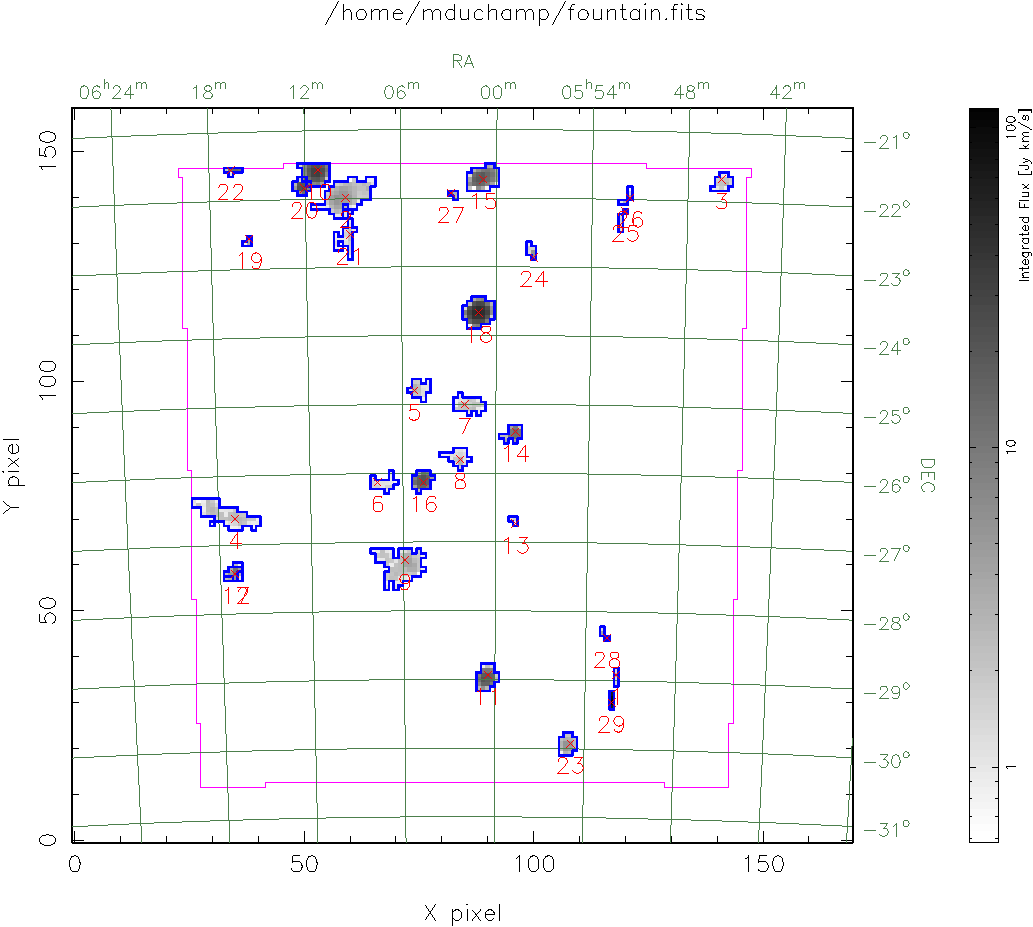
\includegraphics[width=\textwidth]{example_moment_map}
\end{center}
\caption{\footnotesize An example of the moment map created by
  \duchamp. The full extent of the cube is covered, and the 0th moment
  of each object is shown (integrated individually over all the
  detected channels).}
\label{fig-moment}
\end{figure}

Finally, a couple of images are optionally produced: a 0th moment map
of the cube, combining just the detected channels in each object,
showing the integrated flux in grey-scale; and a ``detection image'',
a grey-scale image where the pixel values are the number of channels
that spatial pixel is detected in. In both cases, if
\texttt{drawBorders = true}, a border is drawn around the spatial
extent of each detection. An example moment map is shown in
Fig.~\ref{fig-moment}.  The production or otherwise of these images is
governed by the \texttt{flagMaps} parameter.

The purpose of these images are to provide a visual guide to where the
detections have been made, and, particularly in the case of the moment
map, to provide an indication of the strength of the source. In both
cases, the detections are numbered (in the same sense as the output
list), and the spatial borders are marked out as for the cutout images
in the spectra file. Both these images are saved as postscript files
(given by the parameters \texttt{momentMap} and \texttt{detectionMap}
respectively), with the latter also displayed in a {\sc pgplot}
window (regardless of the state of \texttt{flagMaps}).

\section{Notes and hints on the use of \duchamp}
\label{sec-notes}

In using \duchamp, the user has to make a number of decisions about
the way the program runs. This section is designed to give the user
some idea about what to choose.

The main choice is whether or not to use the wavelet
reconstruction. The main benefits of this are the marked reduction in
the noise level, leading to regularly-shaped detections, and good
reliability for faint sources. The main drawback with its use is the
long execution time: to reconstruct a $170\times160\times1024$
(\hipass) cube often requires three iterations and takes about 20-25
minutes to run completely. Note that this is for the three-dimensional
reconstruction: using \texttt{reconDim=1} makes the reconstruction
quicker (the full program then takes about 6 minutes), but it is still
the largest part of the time.

The searching part of the procedure is much quicker: searching an
un-reconstructed cube leads to execution times of only a couple of
minutes. Alternatively, using the ability to read in previously-saved
reconstructed arrays makes running the reconstruction more than once a
more feasible prospect.

On the positive side, the shape of the detections in a cube that has
been reconstructed will be much more regular and smooth -- the ragged
edges that objects in the raw cube possess are smoothed by the removal
of most of the noise. This enables better determination of the shapes
and characteristics of objects.

A further point to consider when using the reconstruction is that if
the two-dimensional reconstruction is chosen (\texttt{reconDim=2}), it
can be susceptible to edge effects. If the valid area in the cube (\ie
the part that is not BLANK) has non-rectangular edges, the convolution
can produce artefacts in the reconstruction that mimic the edges and
can lead (depending on the selection threshold) to some spurious
sources. Caution is advised with such data -- the user is advised to
check carefully the reconstructed cube for the presence of such
artefacts. Note, however, that the 1- and 3-dimensional
reconstructions are \emph{not} susceptible in the same way, since the
spectral direction does not generally exhibit these BLANK edges, and
so we recommend the use of either of these.

If one chooses the reconstruction method, a further decision is
required on the signal-to-noise cutoff used in determining acceptable
wavelet coefficients. A larger value will remove more noise from the
cube, at the expense of losing fainter sources, while a smaller value
will include more noise, which may produce spurious detections, but
will be more sensitive to faint sources. Values of less than about
$3\sigma$ tend to not reduce the noise a great deal and can lead to
many spurious sources (although this will depend on the nature of the
cube).

When it comes to searching, the FDR method produces more reliable results 
than simple sigma-clipping, particularly in the absence of reconstruction. 
However, it does not work in exactly the way one would expect for a 
given value of \texttt{alpha}. For instance, setting fairly liberal values 
of \texttt{alpha} (say, 0.1) will often lead to a much smaller fraction 
of false detections (\ie much less than 10\%). This is the effect of the 
merging algorithms, that combine the sources after the detection stage,  
and reject detections not meeting the minimum pixel or channel requirements. 
It is thus better to aim for larger \texttt{alpha} values than those derived
from a straight conversion of the desired false detection rate.

Finally, as \duchamp\ is still undergoing development, there are some
elements that are not fully developed. In particular, it is not as
clever as I would like at avoiding interference. The ability to place
requirements on the minimum number of channels and pixels partially
circumvents this problem, but work is being done to make \duchamp\
smarter at rejecting signals that are clearly (to a human eye at
least) interference. See the following section for further
improvements that are planned.

\section{Future Developments}

This is both a list of planned improvements and a wish-list of
features that would be nice to include (but are not planned in the
immediate future). Let me know if there are items not on this list, or
items on the list you would like prioritised.

\begin{itemize}

\item Better determination of the noise characteristics of
  spectral-line cubes, including understanding how the noise is
  generated and developing a model for it. \textbf{Planned.}
  
\item Include more source analysis. Examples could be: shape
  information; measurements of HI mass; more variety of measurements
  of velocity width and profile. \textbf{Some planned.}

\item Provide some indication of the significance of the detection
  (\ie some S/N-like value). \textbf{Planned.}

\item Improved ability to reject interference, possibly on the
  spectral shape of features. \textbf{Planned.}

\item Ability to separate (de-blend) distinct sources that have been
  merged. \textbf{Planned.}

\item Link to lists of possible counterparts (\eg via NED/SIMBAD/other
  VO tools?). \textbf{Wish-list.} 

\item On-line web service interface, so a user can upload a cube and
  get back a source-list. \textbf{Wish-list}.

\item Embed \duchamp\ in a GUI, to move away from the text-based
  interaction. \textbf{Wish-list}.
\end{itemize}


%\bibliographystyle{mn2e}
%\bibliographystyle{abbrvnat}
%\bibliography{mnrasmnemonic,sourceDetection}
\begin{thebibliography}{}

\bibitem[\protect\citeauthoryear{{Calabretta} \& {Greisen}}{{Calabretta} \&
  {Greisen}}{2002}]{calabretta02}
{Calabretta} M.,  {Greisen} E.,  2002, A\&A, 395, 1077

\bibitem[\protect\citeauthoryear{{Greisen} \& {Calabretta}}{{Greisen} \&
  {Calabretta}}{2002}]{greisen02}
{Greisen} E.,  {Calabretta} M.,  2002, A\&A, 395, 1061

\bibitem[\protect\citeauthoryear{{Hanisch}, {Farris}, {Greisen}, {Pence},
  {Schlesinger}, {Teuben}, {Thompson} \& {Warnock}}{{Hanisch}
  et~al.}{2001}]{hanisch01}
{Hanisch} R.,  {Farris} A.,  {Greisen} E.,  {Pence} W.,  {Schlesinger} B.,
  {Teuben} P.,  {Thompson} R.,    {Warnock} A.,  2001, A\&A, 376, 359

\bibitem[\protect\citeauthoryear{{Hopkins}, {Miller}, {Connolly}, {Genovese},
  {Nichol} \& {Wasserman}}{{Hopkins} et~al.}{2002}]{hopkins02}
{Hopkins} A.,  {Miller} C.,  {Connolly} A.,  {Genovese} C.,  {Nichol} R.,
  {Wasserman} L.,  2002, AJ, 123, 1086

\bibitem[\protect\citeauthoryear{Lutz}{Lutz}{1980}]{lutz80}
Lutz R.,  1980, The Computer Journal, 23, 262

\bibitem[\protect\citeauthoryear{{Meyer} et~al.,}{{Meyer}
  et~al.}{2004}]{meyer04:trunc}
{Meyer} M.,  et~al., 2004, MNRAS, 350, 1195

\bibitem[\protect\citeauthoryear{{Miller}, {Genovese}, {Nichol}, {Wasserman},
  {Connolly}, {Reichart}, {Hopkins}, {Schneider} \& {Moore}}{{Miller}
  et~al.}{2001}]{miller01}
{Miller} C.,  {Genovese} C.,  {Nichol} R.,  {Wasserman} L.,  {Connolly} A.,
  {Reichart} D.,  {Hopkins} A.,  {Schneider} J.,    {Moore} A.,  2001, AJ, 122,
  3492

\bibitem[\protect\citeauthoryear{Minchin}{Minchin}{1999}]{minchin99}
Minchin R.,  1999, PASA, 16, 12

\bibitem[\protect\citeauthoryear{Starck \& Murtagh}{Starck \&
  Murtagh}{2002}]{starck02:book}
Starck J.-L.,  Murtagh F.,  2002, {``Astronomical Image and Data Analysis''}.
Springer

\end{thebibliography}


\appendix
\newpage
\section{Obtaining and Installing \duchamp}

The \duchamp\ web page can be found at the following location:\\
\href{http://www.atnf.csiro.au/people/Matthew.Whiting/Duchamp}%
{http://www.atnf.csiro.au/people/Matthew.Whiting/Duchamp}\\
Here you can find a gzipped tar archive of the source code that can be
downloaded and extracted, as well as this User's Guide in postscript
and hyperlinked PDF formats.

\duchamp\ can be built on Unix systems by typing (assuming that the
prompt your terminal provides is a \texttt{> } -- don't type this
character!):
\begin{quote}
\texttt{%
> ./configure\\
> make\\
> make clean (optional -- to remove the object files)}
\end{quote}

Run in this manner, \texttt{configure} should find all the necessary
libraries, but if some libraries have been installed in non-standard
locations, it may fail. In this case, you can specify additional
directories to look in by giving extra command-line arguments. There
are separate options for library files (eg. libcpgplot.a) and header
files (eg. cpgplot.h).

For example, if \textsc{wcslib} had been installed in
\texttt{/home/mduchamp/wcslib}, there are two libraries that are
likely to be in separate subdirectories: \texttt{C/} and
\texttt{pgsbox/}. Each subdirectory needs to be searched for library
and header files, so one could build Duchamp by typing: 
\begin{quote}
\texttt{%
>  ./configure $\backslash$ \\ 
LIBDIRS="/home/mduchamp/wcslib/C /home/mduchamp/wcslib/pgsbox" 
$\backslash$\\
INCDIRS="/home/mduchamp/wcslib/C /home/mduchamp/wcslib/pgsbox"}
\end{quote}
And then just run make in the usual fashion:
\begin{quote}
\texttt{> make}
\end{quote}

This will produce the executable \texttt{Duchamp}. There are two
possible ways to run it. The first is:
\begin{quote}
\texttt{> Duchamp -f [FITS file]}
\end{quote}
where \texttt{[FITS file]} is the file you wish to search. This method
simply uses the default values of all parameters.

The second method allows some determination of the parameter values by
the user. Type:
\begin{quote}
\texttt{> Duchamp -p [parameter file]}
\end{quote}
where \texttt{[parameterFile]} is a file with the input parameters,
including the name of the cube you want to search. There are two
example input files included with the distribution. The smaller one,
\texttt{InputExample}, shows the typical parameters one might want to
set. The large one, \texttt{InputComplete}, lists all possible
parameters that can be entered, and a brief description of them. To
get going quickly, just replace the "your-file-here" in
\texttt{InputExample} with your image name, and type
\begin{quote}
\texttt{> Duchamp -p InputExample}
\end{quote}

The following appendices provide details on the individual parameters,
and show examples of the output files that \duchamp\ produces.

\newpage
\section{Available parameters}
\label{app-param}

The full list of parameters that can be listed in the input file are
given here. If not listed, they take the default value given in
parentheses. Since the order of the parameters in the input file does
not matter, they are grouped here in logical sections.

\subsection*{Input-output related}
\begin{entry}
\item[ImageFile (no default assumed)] The filename of the
  data cube to be analysed.
\item[flagSubsection \texttt{[false]}] A flag to indicate whether one
  wants a subsection of the requested image.
\item[Subsection \texttt{[ [*,*,*] ]}] The requested subsection, which
  should be specified in the format \texttt{[x1:x2,y1:y2,z1:z2]}, where
  the limits are inclusive. If the full range of a dimension is
  required, use a \texttt{*}, \eg if you want the full spectral range of
  a subsection of the image, use \texttt{[30:140,30:140,*]}.
\item[flagReconExists \texttt{[false]}] A flag to indicate whether the
  reconstructed array has been saved by a previous run of \duchamp. If
  set true, the reconstructed array will be read from the file given by
  \texttt{reconFile}, rather than calculated directly.
\item[reconFile (no default assumed)] The FITS file that contains the
  reconstructed array. If \texttt{flagReconExists} is true and this
  parameter is not defined, the default file searched will be
  determined by the \atrous\ parameters (see \S\ref{sec-recon}).
\item[OutFile \texttt{[duchamp-Results.txt]}] The file containing the
  final list of detections. This also records the list of input
  parameters.
\item[SpectraFile \texttt{[duchamp-Spectra.ps]}] The postscript file
  containing the resulting integrated spectra and images of the
  detections. 
\item[flagLog \texttt{[true]}] A flag to indicate whether intermediate
  detections should be logged.
\item[LogFile \texttt{[duchamp-Logfile.txt]}] The file in which intermediate
  detections are logged. These are detections that have not been
  merged. This is primarily for use in debugging and diagnostic
  purposes -- normal use of the program will probably not require
  this.
\item[flagOutputRecon \texttt{[false]}] A flag to say whether or not to
  save the reconstructed cube as a FITS file. The filename will be
  derived from the ImageFile -- the reconstruction of \texttt{image.fits}
  will be saved as \texttt{image.RECON?.fits}, where \texttt{?} stands for
  the value of \texttt{snrRecon} (see below).
\item[flagOutputResid \texttt{[false]}] As for \texttt{flagOutputRecon}, but
  for the residual array -- the difference between the original cube
  and the reconstructed cube. The filename will be \texttt{image.RESID?.fits}.
\item[flagVOT \texttt{[false]}] A flag to say whether to create a VOTable
  file corresponding to the information in \texttt{outfile}. This will be
  an XML file in the Virtual Observatory VOTable format.
\item[votFile \texttt{[duchamp-Results.xml]}] The VOTable file with the
  list of final detections. Some input parameters are also recorded.
\item[flagKarma \texttt{[false]}] A flag to say whether to create a
  Karma annotation file corresponding to the information in
  \texttt{outfile}. This can be used as an overlay for the Karma
  programs such as \texttt{kvis}.
\item[karmaFile \texttt{[duchamp-Results.ann]}] The Karma annotation
  file showing the list of final detections. 
\item[flagMaps \texttt{[true]}] A flag to say whether to save
  postscript files showing the 0th moment map of the whole cube
  (parameter \texttt{momentMap}) and the detection image
  (\texttt{detectionMap}).
\item[momentMap \texttt{[duchamp-MomentMap.ps]}] A postscript file
  containing a map of the 0th moment of the detected sources, as well
  as pixel and WCS coordinates.
\item[detectionMap \texttt{[duchamp-DetectionMap.ps]}] A postscript
  file showing each of the detected objects, coloured in greyscale by
  the number of channels spanned by each pixel. Also shows pixel and WCS
  coordinates.
\end{entry}

\subsection*{Modifying the cube}
\begin{entry}
\item[flagBlankPix \texttt{[true]}] A flag to say whether to remove BLANK
  pixels from the analysis -- these are pixels set to some particular
  value because they fall outside the imaged area.
\item[blankPixValue \texttt{[-8.00061]}] The value of the BLANK pixels,
  if this information is not contained in the FITS header (the usual
  procedure is to obtain this value from the header information -- in
  which case the value set by this parameter is ignored).
\item[flagMW \texttt{[false]}] A flag to say whether to ignore channels
  contaminated by Milky Way (or other) emission -- the searching
  algorithms will not look at these channels.
\item[maxMW \texttt{[112]}] The maximum channel number containing
  ``Milky Way'' emission.
\item[minMW \texttt{[75]}] The minimum channel number containing
  ``Milky Way'' emission. Note that the range specified by
  \texttt{maxMW} and \texttt{minMW} is inclusive.
\item[flagBaseline \texttt{[false]}] A flag to say whether to remove the
  baseline from each spectrum in the cube for the purposes of
  reconstruction and detection.
\end{entry}

\subsection*{Detection related}

\subsubsection*{General detection}
\begin{entry}
\item[flagNegative \texttt{[false]}] A flag to indicate that the features
  being searched for are negative. The cube will be inverted prior to
  searching. 
\item[snrCut \texttt{[3.]}] The cut-off value for thresholding, in terms
  of number of $\sigma$ above the mean.
\item[flagGrowth \texttt{[false]}] A flag indicating whether or not to
  grow the detected objects to a smaller threshold.
\item[growthCut \texttt{[2.]}] The smaller threshold using in growing
  detections. In units of $\sigma$ above the mean.
\end{entry}

\subsubsection*{\Atrous\ reconstruction}
\begin{entry}
\item [flagATrous \texttt{[true]}] A flag indicating whether or not to
  reconstruct the cube using the \atrous\ wavelet
  reconstruction. See \S\ref{sec-recon} for details.
\item[reconDim \texttt{[3]}] The number of dimensions to use in the
  reconstruction. 1 means reconstruct each spectrum separately, 2
  means each channel map is done separately, and 3 means do the whole
  cube in one go.
\item[scaleMin \texttt{[1]}] The minimum wavelet scale to be used in the
  reconstruction. A value of 1 means ``use all scales''.
\item[snrRecon \texttt{[4]}] The thresholding cutoff used in the
  reconstruction -- only wavelet coefficients this many $\sigma$ above
  the mean (or greater) are included in the reconstruction. 
\item[filterCode \texttt{[1]}] The code number of the filter to use in
  the reconstruction. The options are:
  \begin{itemize}
  \item \textbf{1:} B$_3$-spline filter: coefficients = 
    $(\frac{1}{16}, \frac{1}{4}, \frac{3}{8}, \frac{1}{4}, \frac{1}{16})$
  \item \textbf{2:} Triangle filter: coefficients = 
    $(\frac{1}{4}, \frac{1}{2}, \frac{1}{4})$
  \item \textbf{3:} Haar wavelet: coefficients = 
    $(0, \frac{1}{2}, \frac{1}{2})$
  \end{itemize}
\end{entry}

\subsubsection*{FDR method}
\begin{entry}
\item[flagFDR \texttt{[false]}] A flag indicating whether or not to use
  the False Discovery Rate method in thresholding the pixels.
\item[alphaFDR \texttt{[0.01]}] The $\alpha$ parameter used in the FDR
analysis. The average number of false detections, as a fraction of the
total number, will be less than $\alpha$ (see \S\ref{sec-detection}).
\end{entry}

\subsubsection*{Merging detections}
\begin{entry}
\item[minPix \texttt{[2]}] The minimum number of spatial pixels for a single
  detection to be counted.
\item[minChannels \texttt{[3]}] The minimum number of consecutive
  channels that must be present in a detection.
\item[flagAdjacent \texttt{[true]}] A flag indicating whether to use the
  ``adjacent pixel'' criterion to decide whether to merge objects. If
  not, the next two parameters are used to determine whether objects
  are within the necessary thresholds.
\item[threshSpatial \texttt{[3.]}] The maximum allowed minimum spatial
  separation (in pixels) between two detections for them to be merged
  into one. Only used if \texttt{flagAdjacent = false}.
\item[threshVelocity \texttt{[7.]}] The maximum allowed minimum channel
  separation between two detections for them to be merged into
  one. 
\end{entry}

\subsubsection*{Other parameters}
\begin{entry}
\item[spectralMethod \texttt{[peak]}] This indicates which method is used
  to plot the output spectra: \texttt{peak} means plot the spectrum
  containing the detection's peak pixel; \texttt{sum} means sum the
  spectra of each detected spatial pixel, and correct for the beam
  size. Any other choice defaults to \texttt{peak}.
\item[spectralUnits \texttt{[km/s]}] The user can specify the units of
  the spectral axis. Assuming the WCS of the FITS file is valid, the
  spectral axis is transformed into velocity, and put into these units
  for all output and for calculations such as the integrated flux of a
  detection.
\item[drawBorders \texttt{[true]}] A flag indicating whether borders
  are to be drawn around the detected objects in the moment maps
  included in the output (see for example Fig.~\ref{fig-spect}).
\item[verbose \texttt{[true]}] A flag indicating whether to print the
  progress of computationally-intensive algorithms (such as the
  searching and merging) to screen.
\end{entry}


\newpage
\section{Example parameter files}
\label{app-input}

This is what a typical parameter file would look like.

\begin{verbatim}
imageFile       /DATA/SITAR_1/whi550/cubes/H201_abcde_luther_chop.fits
logFile         logfile.txt
outFile         results.txt
spectraFile     spectra.ps
flagSubsection  false
flagOutputRecon false
flagOutputResid 0
flagBlankPix    1
flagMW          1
minMW           75
maxMW           112
minPix          3
flagGrowth      1
growthCut       1.5
flagATrous      0
scaleMin        1
snrRecon        4
flagFDR         1
alphaFDR        0.1
numPixPSF       20
snrCut          3
threshSpatial   3
threshVelocity  7
\end{verbatim}

Note that, as in this example, the flag parameters can be entered as
strings (true/false) or integers (1/0). Also, note that it is not
necessary to include all these parameters in the file, only those that
need to be changed from the defaults (as listed in
Appendix~\ref{app-param}), which in this case would be very few. A
minimal parameter file might look like:
\begin{verbatim}
imageFile       /DATA/SITAR_1/whi550/cubes/H201_abcde_luther_chop.fits
flagLog         false
snrRecon        3
snrCut          2.5
minChannels     4
\end{verbatim}
This will reconstruct the cube with a lower SNR value than the
default, select objects at a lower threshold,  with a looser minimum
channel requirement, and not keep a log of the intermediate
detections. 

The following page demonstrates how the parameters are presented to the 
user, both on the screen at execution time, and in the output and log 
files. On each line, there is a description on the parameter, the relevant 
parameter name that is used in the input file (if there is one that the 
user can enter), and the value of the parameter being used. 
\newpage
\begin{landscape}
Typical presentation of parameters in output and log files:  
\begin{verbatim}
---- Parameters ----
Image to be analysed.........................[imageFile]  =  input.fits
Intermediate Logfile...........................[logFile]  =  duchamp-Logfile.txt	  
Final Results file.............................[outFile]  =  duchamp-Results.txt	  
Spectrum file..............................[spectraFile]  =  duchamp-Spectra.ps	  
0th Moment Map...............................[momentMap]  =  duchamp-MomentMap.ps
Detection Map.............................[detectionMap]  =  duchamp-DetectionMap.ps
Saving reconstructed cube?.............[flagoutputrecon]  =  false
Saving residuals from reconstruction?..[flagoutputresid]  =  false
------
Searching for Negative features?..........[flagNegative]  =  false
Fixing Blank Pixels?......................[flagBlankPix]  =  true
Blank Pixel Value.......................................  =  -8.00061
Removing Milky Way channels?....................[flagMW]  =  true
Milky Way Channels.......................[minMW - maxMW]  =  75-112
Beam Size (pixels)......................................  =  10.1788
Removing baselines before search?.........[flagBaseline]  =  false
Minimum # Pixels in a detection.................[minPix]  =  2
Minimum # Channels in a detection..........[minChannels]  =  3
Growing objects after detection?............[flagGrowth]  =  false
Using A Trous reconstruction?...............[flagATrous]  =  true
Number of dimensions in reconstruction........[reconDim]  =  3
Minimum scale in reconstruction...............[scaleMin]  =  1
SNR Threshold within reconstruction...........[snrRecon]  =  4
Filter being used for reconstruction........[filterCode]  =  1 (B3 spline function)
Using FDR analysis?............................[flagFDR]  =  false
SNR Threshold...................................[snrCut]  =  3
Using Adjacent-pixel criterion?...........[flagAdjacent]  =  true
Max. velocity separation for merging....[threshVelocity]  =  7
Method of spectral plotting.............[spectralMethod]  =  peak
\end{verbatim}

\newpage
\section{Example results file}
\label{app-output}
This the typical content of an output file, after running \duchamp\
with the parameters illustrated on the previous page. 

{\scriptsize 
  \begin{verbatim}
Results of the \duchamp\ source finder: Tue May 23 14:51:38 2006
---- Parameters ----
      (... omitted for clarity -- see previous page for examples...)
--------------------
Total number of detections = 25
--------------------
------------------------------------------------------------------------------------------------------------------------------------------------------
 Obj#       Name     X     Y     Z           RA          DEC      VEL     w_RA    w_DEC   w_VEL     F_int    F_peak  X1  X2  Y1  Y2  Z1  Z2  Npix Flag
                                                               [km/s] [arcmin] [arcmin]  [km/s] [Jy km/s] [Jy/beam]                         [pix]     
------------------------------------------------------------------------------------------------------------------------------------------------------
    1 J0618-2532  30.2  86.0 113.3  06:18:12.54 -25:32:44.79  208.502    45.17    34.61  26.383    24.394     0.350  25  35  82  90 112 114   137    E
    2 J0609-2156  59.5 140.6 114.6  06:09:19.66 -21:56:31.20  225.572    44.39    31.47  65.957    16.128     0.213  55  65 137 144 113 118   153     
    3 J0545-2143 141.2 143.2 114.8  05:45:51.71 -21:43:36.20  228.470    19.61    16.66  26.383     2.412     0.090 139 143 142 145 114 116    29     
    4 J0617-2633  33.3  70.8 115.6  06:17:25.52 -26:33:33.83  238.736    65.02    30.10  26.383     9.776     0.117  26  41  68  75 115 117   104    E
    5 J0601-2500  86.2  94.9 117.9  06:01:39.54 -25:00:32.46  269.419    27.99    24.02  26.383     3.920     0.124  83  89  92  97 117 119    44     
    6 J0602-2547  84.0  83.1 118.0  06:02:18.29 -25:47:31.69  270.319    20.01    19.99  26.383     2.999     0.118  82  86  81  85 117 119    34     
    7 J0547-2448 133.0  97.2 118.7  05:47:52.53 -24:48:38.16  279.113    19.72    12.54  26.383     1.474     0.074 131 135  96  98 118 120    21     
    8 J0606-2719  71.1  60.0 121.3  06:06:10.99 -27:19:48.61  314.090    52.36    39.59  39.574    14.268     0.150  65  77  55  64 120 123   154     
    9 J0611-2137  52.4 145.3 162.5  06:11:20.92 -21:37:29.57  857.955    32.39    23.49 118.722    43.178     0.410  49  56 142 147 158 167   265    E
   10 J0600-2859  89.7  35.3 202.4  06:00:34.08 -28:59:00.43 1383.160    23.93    24.10 171.487    24.439     0.173  87  92  33  38 196 209   271     
   11 J0558-2638  95.4  70.3 223.1  05:58:53.03 -26:38:45.91 1656.140    11.93    12.07  92.339     1.045     0.063  94  96  69  71 220 227    18     
   12 J0617-2723  34.7  58.3 227.4  06:17:07.07 -27:23:50.65 1712.868    16.75    23.53 290.209     8.529     0.093  33  36  56  61 215 237   118     
   13 J0558-2525  95.8  88.6 231.7  05:58:49.27 -25:25:33.60 1770.134    27.87    24.16 237.444    12.863     0.115  92  98  86  91 221 239   175     
   14 J0600-2141  88.8 144.4 232.5  06:00:54.02 -21:41:57.06 1780.188    27.96    24.13 224.252    30.743     0.166  86  92 142 147 222 239   344    E
   15 J0615-2634  40.0  70.8 232.6  06:15:25.50 -26:34:20.04 1782.214    12.44    15.69  52.765     2.084     0.068  39  41  69  72 231 235    31     
   16 J0604-2606  76.0  78.4 233.0  06:04:41.13 -26:06:21.19 1787.226    24.13    23.87 211.061    23.563     0.155  73  78  76  81 225 241   278     
   17 J0601-2340  87.9 114.9 235.8  06:01:08.83 -23:40:19.37 1824.122    31.95    28.09 237.444    82.380     0.297  85  92 112 118 227 245   647     
   18 J0615-2235  38.2 130.5 254.5  06:15:32.09 -22:35:37.24 2070.934    12.29    11.70 105.531     1.555     0.070  37  39 129 131 249 257    24     
   19 J0617-2305  31.4 122.8 258.1  06:17:33.45 -23:05:28.94 2118.752    12.34    11.65  26.383     1.022     0.062  30  32 122 124 257 259    16     
   20 J0612-2149  49.6 142.2 270.3  06:12:11.04 -21:49:29.72 2279.926    16.27    15.73 395.740    15.156     0.101  48  51 141 144 257 287   204     
   21 J0616-2133  35.3 146.0 300.6  06:16:15.78 -21:33:09.69 2679.148    20.22     7.47 224.252     3.014     0.127  33  37 145 146 294 311    28    E
   22 J0555-2956 107.3  20.9 367.6  05:55:08.02 -29:56:09.08 3562.236    19.71    20.30  39.574     5.891     0.169 105 109  19  23 366 369    58     
   23 J0557-2246  99.8 128.2 434.0  05:57:43.77 -22:46:42.95 4438.776    11.88    16.12 105.531     1.703     0.167  99 101 127 130 430 438    17    N
   24 J0616-2648  38.1  67.2 546.8  06:16:02.10 -26:48:35.49 5926.464    12.35    11.67  26.383     1.276     0.064  37  39  66  68 546 548    18     
   25 J0552-2916 117.0  30.5 727.0  05:52:13.64 -29:16:58.02 8303.952    11.59    20.25 303.400    35.523     0.479 116 118  28  32 716 739   111     
  \end{verbatim}
}
Note that the
width of the table can make it hard to read. A good trick for those
using UNIX/Linux is to make use of the \texttt{a2ps} command. The
following works well, producing a postscript file \texttt{results.ps}:
\\\verb|a2ps -1 -r -f8 -o duchamp-Results.ps duchamp-Results.txt|

%\end{landscape}

\newpage
\section{Example VOTable output}
\label{app-votable}
This is part of the VOTable, in XML format, corresponding to the
output file in Appendix~\ref{app-output} (the indentation has been
removed to make it fit on the page).

%\begin{landscape}
{\scriptsize
  \begin{verbatim}
<?xml version="1.0"?>
<VOTABLE version="1.1" xmlns:xsi="http://www.w3.org/2001/XMLSchema-instance"
 xsi:noNamespaceSchemaLocation="http://www.ivoa.net/xml/VOTable/VOTable/v1.1">
<COOSYS ID="J2000" equinox="J2000." epoch="J2000." system="eq_FK5"/>
<RESOURCE name="Duchamp Output">
<TABLE name="Detections">
<DESCRIPTION>Detected sources and parameters from running the Duchamp source finder.</DESCRIPTION>
<PARAM name="FITS file" datatype="char" ucd="meta.file;meta.fits" value="/DATA/SITAR_1/whi550/cubes/H201_abcde_luther_chop.fits"/>
<PARAM name="Threshold" datatype="float" ucd="stat.snr" value="2.5">
<PARAM name="ATrous note" datatype="char" ucd="meta.note" value="The a trous reconstruction method was used, with the following parameters.">
<PARAM name="ATrous Dimension" datatype="int" ucd="meta.code;stat" value="3">
<PARAM name="ATrous Cut" datatype="float" ucd="stat.snr" value="4">
<PARAM name="ATrous Minimum Scale" datatype="int" ucd="stat.param" value="1">
<PARAM name="ATrous Filter" datatype="char" ucd="meta.code;stat" value="B3 spline function">
<FIELD name="ID" ID="col1" ucd="meta.id" datatype="int" width="4"/>
<FIELD name="Name" ID="col2" ucd="meta.id;meta.main" datatype="char" arraysize="14"/>
<FIELD name="RA" ID="col3" ucd="pos.eq.ra;meta.main" ref="J2000" datatype="float" width="10" precision="6" unit="deg"/>
<FIELD name="Dec" ID="col4" ucd="pos.eq.dec;meta.main" ref="J2000" datatype="float" width="10" precision="6" unit="deg"/>
<FIELD name="w_RA" ID="col3" ucd="phys.angSize;pos.eq.ra" ref="J2000" datatype="float" width="7" precision="2" unit="arcmin"/>
<FIELD name="w_Dec" ID="col4" ucd="phys.angSize;pos.eq.dec" ref="J2000" datatype="float" width="7" precision="2" unit="arcmin"/>
<FIELD name="Vel" ID="col4" ucd="phys.veloc;src.dopplerVeloc" datatype="float" width="9" precision="3" unit="km/s"/>
<FIELD name="w_Vel" ID="col4" ucd="phys.veloc;src.dopplerVeloc;spect.line.width" datatype="float" width="8" precision="3" unit="km/s"/>
<FIELD name="Integrated_Flux" ID="col4" ucd="phys.flux;spect.line.intensity" datatype="float" width="10" precision="3" unit="km/s"/>
<DATA>
<TABLEDATA>
<TR>
<TD>   1</TD><TD> J0609-2200</TD><TD> 92.410416</TD><TD>-22.013390</TD><TD>  48.50</TD><TD>  39.42</TD><TD>  213.061</TD><TD>  65.957</TD><TD>    17.572</TD>
</TR>
<TR>
<TD>   2</TD><TD> J0608-2605</TD><TD> 92.042633</TD><TD>-26.085157</TD><TD>  44.47</TD><TD>  39.47</TD><TD>  233.119</TD><TD>  39.574</TD><TD>     4.144</TD>
</TR>
<TR>
<TD>   3</TD><TD> J0606-2724</TD><TD> 91.637840</TD><TD>-27.412022</TD><TD>  52.48</TD><TD>  47.57</TD><TD>  302.213</TD><TD>  39.574</TD><TD>    17.066</TD>
</TR>
(... table truncated for clarity ...)
</TABLEDATA>
</DATA>
</TABLE>
</RESOURCE>
</VOTABLE>
  \end{verbatim}
}
\end{landscape}

\newpage
\section{Example Karma Annotation File output}
\label{app-karma}

This is the format of the Karma Annotation file, showing the locations
of the detected objects. This can be loaded by the plotting tools of
the Karma package (for instance, \texttt{kvis}) as an overlay on the FITS
file.

\begin{verbatim}
# Duchamp Source Finder results for 
#  cube /DATA/SITAR_1/whi550/cubes/H201_abcde_luther_chop.fits
COLOR RED
COORD W
CIRCLE 92.3376 -21.9475 0.403992
TEXT 92.3376 -21.9475 1
CIRCLE 91.9676 -26.0193 0.37034
TEXT 91.9676 -26.0193 2
CIRCLE 91.5621 -27.3459 0.437109
TEXT 91.5621 -27.3459 3
CIRCLE 92.8285 -21.6344 0.269914
TEXT 92.8285 -21.6344 4
CIRCLE 90.1381 -28.9838 0.234179
TEXT 90.1381 -28.9838 5
CIRCLE 89.72 -26.6513 0.132743
TEXT 89.72 -26.6513 6
CIRCLE 94.2743 -27.4003 0.195175
TEXT 94.2743 -27.4003 7
CIRCLE 92.2739 -21.6941 0.134538
TEXT 92.2739 -21.6941 8
CIRCLE 89.7133 -25.4259 0.232252
TEXT 89.7133 -25.4259 9
CIRCLE 90.2206 -21.6993 0.266247
TEXT 90.2206 -21.6993 10
CIRCLE 93.8581 -26.5766 0.163153
TEXT 93.8581 -26.5766 11
CIRCLE 91.176 -26.1064 0.234356
TEXT 91.176 -26.1064 12
CIRCLE 90.2844 -23.6716 0.299509
TEXT 90.2844 -23.6716 13
CIRCLE 93.8774 -22.581 0.130925
TEXT 93.8774 -22.581 14
CIRCLE 94.3882 -23.0934 0.137108
TEXT 94.3882 -23.0934 15
CIRCLE 93.0491 -21.8223 0.202928
TEXT 93.0491 -21.8223 16
CIRCLE 94.0685 -21.5603 0.168456
TEXT 94.0685 -21.5603 17
CIRCLE 86.0568 -27.6095 0.101113
TEXT 86.0568 -27.6095 18
CIRCLE 88.7932 -29.9453 0.202624
TEXT 88.7932 -29.9453 19
\end{verbatim}

\newpage
\section{Robust statistics for a Normal distribution}
\label{app-madfm}

The Normal, or Gaussian, distribution for mean $\mu$ and standard
deviation $\sigma$ can be written as 
\[ 
f(x) = \frac{1}{\sqrt{2\pi\sigma^2}}\ e^{-(x-\mu)^2/2\sigma^2}.
 \]

When one has a purely Gaussian signal, it is straightforward to
estimate $\sigma$ by calculating the standard deviation (or rms) of
the data. However, if there is a small amount of signal present on top
of Gaussian noise, and one wants to estimate the $\sigma$ for the
noise, the presence of the large values from the signal can bias the
estimator to higher values.

An alternative way is to use the median ($m$) and median absolute deviation
from the median ($s$) to estimate $\mu$ and $\sigma$. The median is the
middle of the distribution, defined for a continuous distribution by
\[
\int_{-\infty}^{m} f(x) \diff x = \int_{m}^{\infty} f(x) \diff x.
\]
From symmetry, we quickly see that for the continuous Normal
distribution, $m=\mu$. We consider the case henceforth of $\mu=0$,
without loss of generality.

To find $s$, we find the distribution of the absolute deviation from
the median, and then find the median of that distribution. This
distribution is given by
\begin{eqnarray*}
g(x) &= &{\mbox{\rm distribution of }} |x|\\
     &= &f(x) + f(-x),\ x\ge0\\
     &= &\sqrt{\frac{2}{\pi\sigma^2}}\, e^{-x^2/2\sigma^2},\ x\ge0.
\end{eqnarray*}
So, the median absolute deviation from the median, $s$, is given by
\[
\int_{0}^{s} g(x) \diff x = \int_{s}^{\infty} g(x) \diff x.
\]
Now, $\int_{0}^{\infty}e^{-x^2/2\sigma^2} \diff x = \sqrt{\pi\sigma^2/2}$, and
so $\int_{s}^{\infty} e^{-x^2/2\sigma^2} \diff x =
\sqrt{\pi\sigma^2/2} - \int_{0}^{s} e^{-\frac{x^2}{2\sigma^2}} \diff x
$. Hence, to find $s$ we simply solve the following equation (setting $\sigma=1$ for
simplicity -- equivalent to stating $x$ and $s$ in units of $\sigma$):
\[
\int_{0}^{s}e^{-x^2/2} \diff x - \sqrt{\pi/8} = 0.
\]
This is hard to solve analytically (no nice analytic solution exists
for the finite integral that I'm aware of), but straightforward to
solve numerically, yielding the value of $s=0.6744888$. Thus, to
estimate $\sigma$ for a Normally distributed data set, one can calculate
$s$, then divide by 0.6744888 (or multiply by 1.4826042) to obtain the
correct estimator.

Note that this is different to solutions quoted elsewhere,
specifically in \citet{meyer04:trunc}, where the same robust estimator
is used but with an incorrect conversion to standard deviation -- they
assume $\sigma = s\sqrt{\pi/2}$. This, in fact, is the conversion used
to convert the \emph{mean} absolute deviation from the mean to the
standard deviation. This means that the cube noise in the \hipass\
catalogue (their parameter Rms$_{\rm cube}$) should be 18\% larger
than quoted.

\section{How Gaussian noise changes with wavelet scale.}
\label{app-scaling}

The key element in the wavelet reconstruction of an array is the
thresholding of the individual wavelet coefficient arrays. This is
usually done by choosing a level to be some number of standard
deviations above the mean value.

However, since the wavelet arrays are produced by convolving the input
array by an increasingly large filter, the pixels in the coefficient
arrays become increasingly correlated as the scale of the filter
increases. This results in the measured standard deviation from a
given coefficient array decreasing with increasing scale. To calculate
this, we need to take into account how many other pixels each pixel in
the convolved array depends on.

To demonstrate, suppose we have a 1-D array with $N$ pixel values
given by $F_i,\ i=1,...,N$, and we convolve it with the B$_3$-spline
filter, defined by the set of coefficients
$\{1/16,1/4,3/8,1/4,1/16\}$. The flux of the $i$th pixel in the
convolved array will be
\[
F'_i = \frac{1}{16}F_{i-2} + \frac{1}{4}F_{i-1} + \frac{3}{8}F_{i}
+ \frac{1}{4}F_{i+1} + \frac{1}{16}F_{i+2}
\]
and the flux of the corresponding pixel in the wavelet array will be 
\[
W'_i = F_i - F'_i = \frac{-1}{16}F_{i-2} - \frac{1}{4}F_{i-1} + \frac{5}{8}F_{i}
- \frac{1}{4}F_{i+1} - \frac{1}{16}F_{i+2}
\]
Now, assuming each pixel has the same standard deviation
$\sigma_i=\sigma$, we can work out the standard deviation for the
wavelet array:
\[
\sigma'_i = \sigma \sqrt{\left(\frac{1}{16}\right)^2 + \left(\frac{1}{4}\right)^2
  + \left(\frac{5}{8}\right)^2 + \left(\frac{1}{4}\right)^2 + \left(\frac{1}{16}\right)^2}
          = 0.72349\ \sigma
\]
Thus, the first scale wavelet coefficient array will have a standard
deviation of 72.3\% of the input array. This procedure can be followed
to calculate the necessary values for all scales, dimensions and
filters used by \duchamp.

Calculating these values is clearly a critical step in performing the
reconstruction. \citet{starck02:book} did so by simulating data sets
with Gaussian noise, taking the wavelet transform, and measuring the
value of $\sigma$ for each scale. We take a different approach, by
calculating the scaling factors directly from the filter coefficients
by taking the wavelet transform of an array made up of a 1 in the
central pixel and 0s everywhere else. The scaling value is then
derived by taking the square root of the sum (in quadrature) of all
the wavelet coefficient values at each scale. We give the scaling
factors for the three filters available to \duchamp\ on the following
page. These values are hard-coded into \duchamp, so no on-the-fly
calculation of them is necessary.

Memory limitations prevent us from calculating factors for large
scales, particularly for the three-dimensional case (hence the --
symbols in the tables). To calculate factors for
higher scales than those available, we note the following
relationships apply for large scales to a sufficient level of precision:
\begin{itemize}
\item 1-D: factor(scale $i$) = factor(scale $i-1$)$/\sqrt{2}$.
\item 2-D: factor(scale $i$) = factor(scale $i-1$)$/2$.
\item 1-D: factor(scale $i$) = factor(scale $i-1$)$/\sqrt{8}$.
\end{itemize}

\newpage
\begin{itemize}
\item \textbf{B$_3$-Spline Function:} $\{1/16,1/4,3/8,1/4,1/16\}$

\begin{tabular}{llll}
Scale & 1 dimension      & 2 dimension     & 3 dimension\\ \hline
1     & 0.723489806      & 0.890796310     & 0.956543592\\
2     & 0.285450405	 & 0.200663851	   & 0.120336499\\
3     & 0.177947535	 & 0.0855075048	   & 0.0349500154\\
4     & 0.122223156	 & 0.0412474444	   & 0.0118164242\\
5     & 0.0858113122	 & 0.0204249666	   & 0.00413233507\\
6     & 0.0605703043	 & 0.0101897592	   & 0.00145703714\\
7     & 0.0428107206	 & 0.00509204670   & 0.000514791120\\
8     & 0.0302684024	 & 0.00254566946   & --\\
9     & 0.0214024008	 & 0.00127279050   & --\\
10    & 0.0151336781	 & 0.000636389722  & --\\
11    & 0.0107011079	 & 0.000318194170  & --\\
12    & 0.00756682272	 & --		   & --\\
13    & 0.00535055108	 & --		   & --\\
%14    & 0.00378341085	 & --		   & --\\
%15    & 0.00267527545	 & --		   & --\\
%16    & 0.00189170541	 & --		   & --\\
%17    & 0.00133763772	 & --		   & --\\
%18    & 0.000945852704   & --		   & --
\end{tabular}

\item \textbf{Triangle Function:} $\{1/4,1/2,1/4\}$

\begin{tabular}{llll}
Scale & 1 dimension      & 2 dimension     & 3 dimension\\ \hline
1     & 0.612372436      & 0.800390530     & 0.895954449  \\
2     & 0.330718914	 & 0.272878894     & 0.192033014\\
3     & 0.211947812	 & 0.119779282     & 0.0576484078\\
4     & 0.145740298	 & 0.0577664785    & 0.0194912393\\
5     & 0.102310944	 & 0.0286163283    & 0.00681278387\\
6     & 0.0722128185	 & 0.0142747506    & 0.00240175885\\
7     & 0.0510388224	 & 0.00713319703   & 0.000848538128 \\
8     & 0.0360857673	 & 0.00356607618   & 0.000299949455 \\
9     & 0.0255157615	 & 0.00178297280   & -- \\
10    & 0.0180422389	 & 0.000891478237  & --  \\
11    & 0.0127577667	 & 0.000445738098  & --  \\
12    & 0.00902109930	 & 0.000222868922  & --  \\
13    & 0.00637887978	 & --		   & -- \\
%14   & 0.00451054902	 & --		   & -- \\
%15   & 0.00318942978	 & --		   & -- \\
%16   & 0.00225527449	 & --		   & -- \\
%17   & 0.00159471988	 & --		   & -- \\
%18   & 0.000112763724	 & --		   & -- 

\end{tabular}

\item \textbf{Haar Wavelet:} $\{0,1/2,1/2\}$

\begin{tabular}{llll}
Scale & 1 dimension      & 2 dimension     & 3 dimension\\ \hline
1     & 0.707167810      & 0.433012702     & 0.935414347 \\
2     & 0.500000000	 & 0.216506351     & 0.330718914\\
3     & 0.353553391	 & 0.108253175     & 0.116926793\\
4     & 0.250000000	 & 0.0541265877    & 0.0413398642\\
5     & 0.176776695	 & 0.0270632939    & 0.0146158492\\
6     & 0.125000000	 & 0.0135316469    & 0.00516748303

\end{tabular}


\end{itemize}

\end{document}
